\input{../YKY-preamble}

\newcommand{\ovalA}{\; \vcenter{\hbox{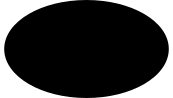
\includegraphics[decodearray={0.4 1 1.0 1 0.4 1}]{oval.png}}} \;}
\newcommand{\ovalB}{\; \vcenter{\hbox{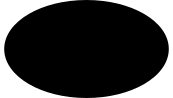
\includegraphics[decodearray={1.0 1 0.4 1 0.4 1}]{oval.png}}} \;}
\newcommand{\ovalC}{\; \vcenter{\hbox{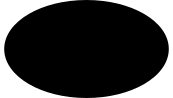
\includegraphics[decodearray={0.9 1 0.8 1 0.4 1}]{oval.png}}} \;}
\newcommand{\ovalD}{\; \vcenter{\hbox{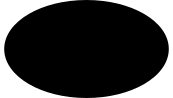
\includegraphics[decodearray={0.75 1 0.75 1 1 1}]{oval.png}}} \;}

\title{Learning inside the Rete algorithm}

\author{YKY (Yan King Yin) \\ {\footnotesize general.intelligence@gmail.com}}

\begin{document}

	\setlength{\parindent}{0pt}
	\setlength{\parskip}{2.8ex plus0.8ex minus0.8ex}
	
	\maketitle
	
\begin{abstract}
\end{abstract}

\section{Introduction to the Rete algorithm}

The general form of a \textbf{production rule} is like this:
\begin{equation}
\overbrace{\ovalA \wedge \ovalA \wedge \ovalA ....}^{\mbox{condition}} \rightarrow \overbrace{\ovalB}^{\mbox{action}}
\end{equation}
where $\wedge$ denotes logical conjunction (AND).

Typically, we would be trying to match a relatively small number of \textbf{facts} (that represent the current \textbf{state}, or \textbf{working memory}) against a very large number of \textbf{rules}:
\begin{equation}
\overbrace{\scalebox{0.7}{\parbox{9em}{.... $\ovalC \ovalC \ovalC$}}}^{\mbox{queue of WMEs}} \quad \mbox{ match against } \quad
\scalebox{0.7}{\parbox{0.3\linewidth}{
\begin{align}
\ovalA \ovalA \ovalA .... \rightarrow \ovalB \nonumber \\
\ovalA \ovalA \ovalA .... \rightarrow \ovalB \nonumber \\
\ovalA \ovalA \ovalA .... \rightarrow \ovalB \nonumber \\
\ovalA \ovalA \ovalA .... \rightarrow \ovalB \nonumber \\
.... \quad .... \quad .... \quad .... \quad \quad \nonumber \\
\ovalA \ovalA \ovalA .... \rightarrow \ovalB \nonumber
\end{align}
}}
\label{eqn:rules-matching}
\end{equation}
where $\ovalC$ = WME = working memory element = fact = \textbf{grounded} logic formula = formula not containing variables.

Obviously, if the number of rules is large, it would be time-consuming to \uline{test each rule one by one} to see if they apply.

It would be much more efficient if we could look at each $\ovalC$ and immediately see which rule(s) may apply to it.  This is the idea behind Rete.  

In other words, we want to \textit{compile} the rule conditions $\ovalA$ into a \textbf{decision tree}:
\begin{equation}
\begin{tikzcd}[column sep = 7em]
\scalebox{0.7}{\parbox{0.3\linewidth}{
		\begin{align}
		\ovalA \ovalA \ovalA ....  \nonumber \\
		\ovalA \ovalA \ovalA ....  \nonumber \\
		\ovalA \ovalA \ovalA ....  \nonumber \\
		.... \quad .... \quad .... \quad \quad \nonumber \\
		\ovalA \ovalA \ovalA ....  \nonumber
		\end{align}
}}
\arrow[r, Rightarrow, "\mbox{Rete algorithm}"] & \quad  \vcenter{\hbox{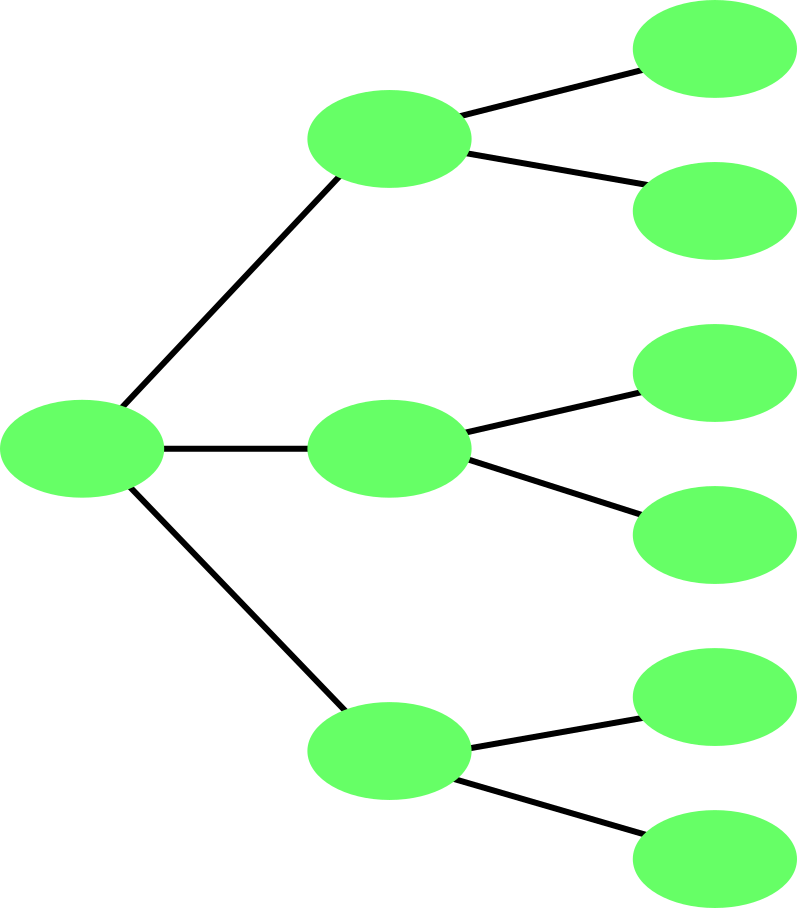
\includegraphics[scale=0.7]{decision-tree.png}}}
\end{tikzcd}
\label{eqn:rete-process}
\end{equation}
The actions $\ovalB$ of the rules do not figure in the decision process.

\subsection{How the Rete graph is constructed}

To construct the decision tree in (\ref{eqn:rete-process}), it may appear that we just need to ``collect like items'', but this would be wrong due to a peculiarity of \textbf{predicate logic}.

That is, there exist \textbf{linkages} across atoms in a conjunction:
\begin{equation}
\forall X \; \forall Y \; \forall Z.  \quad \text{father}({\color{red}X} \tikzmark{p}, {\color{red}Y} \tikzmark{y}) \wedge \mbox{father}({\color{red}Y} \tikzmark{q}, {\color{red}Z} \tikzmark{r}) \rightarrow \text{grandfather}({\color{red}X} \tikzmark{x}, {\color{red}Z} \tikzmark{z}) 
\begin{tikzpicture}[overlay,remember picture,distance=1.1cm]
\draw[-,red, transform canvas={shift={(-5pt,10pt)}}, out=135,in=45] (x.center) to (p.center);
\draw[-,red, transform canvas={shift={(-5pt,-3pt)}}, out=-20,in=210] (y.center) to (q.center);
\draw[-,red, transform canvas={shift={(-5pt,-3pt)}}, out=-25,in=215] (r.center) to (z.center);
\end{tikzpicture}
\label{linkage-father}
\end{equation}
For example, the variable $X$ in 2 different \textbf{positions} must be substituted with the \textit{same} object, otherwise the logic formula is not satisfied.

Rete's idea is to \textit{decompose} each condition $\ovalA$ \uline{into 2 parts}:
\begin{itemize}
	\item one pertaining to the \textbf{internal} structure (``schema'') of the condition itself
	\item one pertaining to the \textbf{inter-relations} between this condition and the others in the conjunction (the ``linkages'')
\end{itemize}
This gives rise to the famous \textbf{alpha} and \textbf{beta} nodes:
\begin{equation}
\ovalA = \alpha\mbox{-condition} \; \wedge \; \beta\mbox{-condition(s)} 
\end{equation}

Each $\alpha$-node is responsible for \uline{matching only 1 atom} in the conjunction:
\begin{equation}
\overbrace{\ovalA}^{\alpha_1} \wedge \overbrace{\ovalA}^{\alpha_2} \wedge \overbrace{\ovalA}^{\alpha_3} .... \rightarrow \ovalB
\end{equation}

A $\beta$-node is responsible for the \uline{relations between the latest atom and the previous atoms}:
\begin{equation}
\overbrace{ \overbrace{ \overbrace{ \ovalA }^{\beta_1} \wedge \ovalA}^{\beta_2} \wedge \ovalA}^{\beta_3} .... \rightarrow \ovalB
\end{equation}
where $\beta_1$ is empty as it contains only 1 atom.

So the conditions of a rule are re-structured as a chain as follows:
\begin{equation}
\vcenter{\hbox{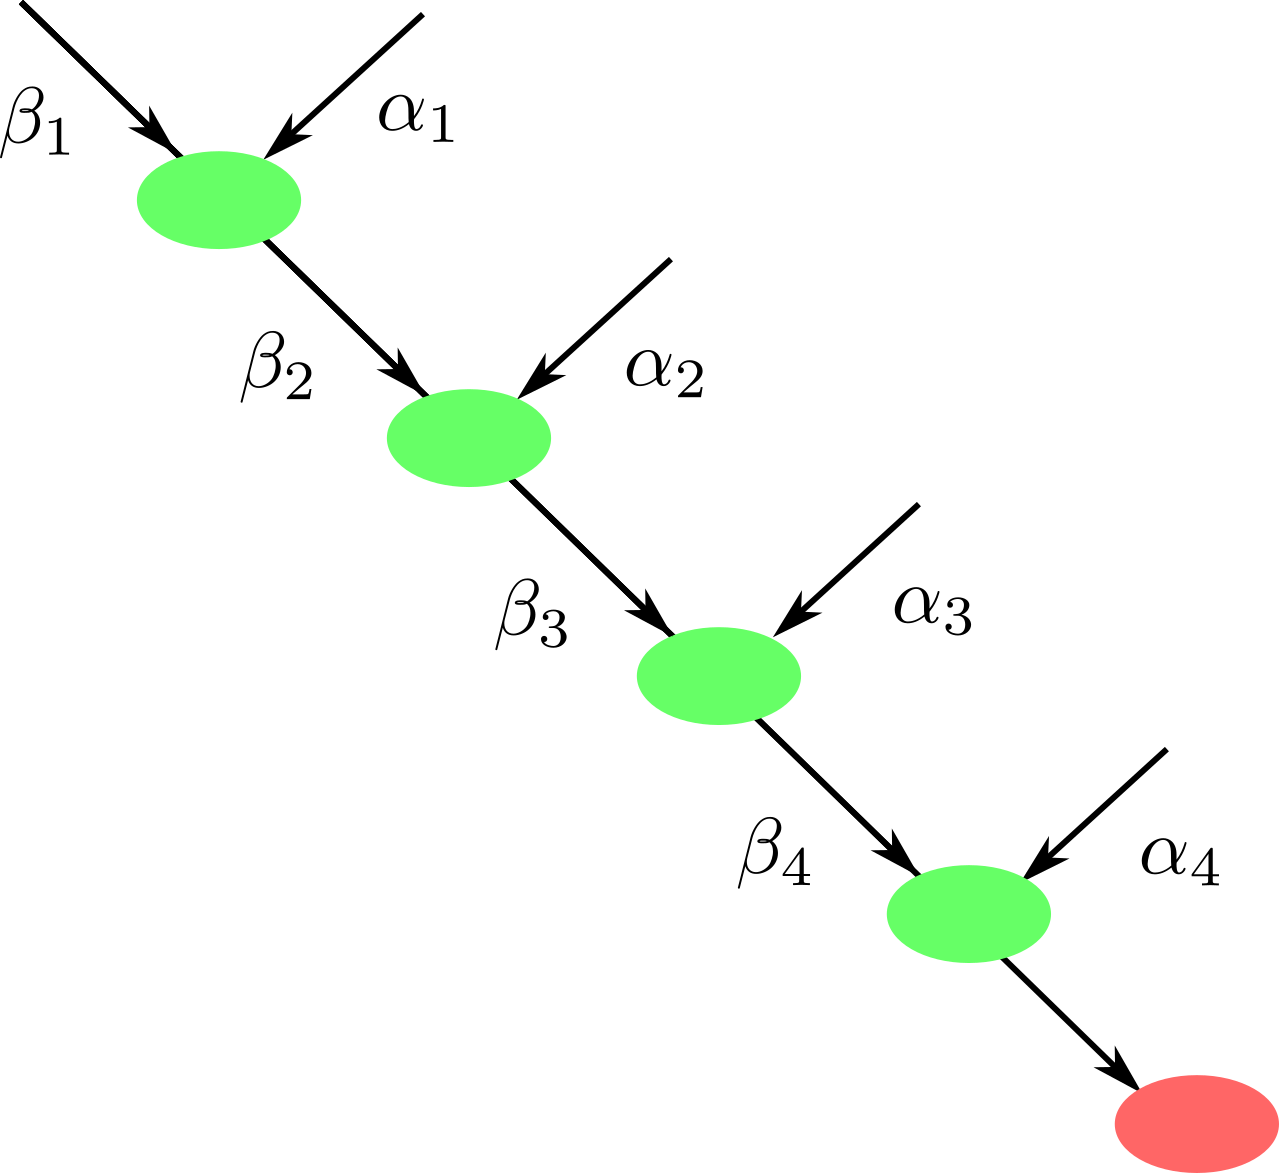
\includegraphics[scale=1]{rete-chain.png}}}
\label{rete-chains}
\end{equation}

Now that all the rules are converted into such chains as (\ref{rete-chains}), the Rete decision network can be constructed simply by \uline{identifying common nodes}.

My presentation may be slightly different from those found on the internet, but I guess the main idea is the same.

\section{Learning inside Rete}

The Rete network completely replaces the set of rules, so we no longer need the latter.  In AI applications, the rules don't even exist initially.  This means that we could learn the Rete network directly.  What is the advantage, you may ask?

\subsection{Relation to deep learning}

The standard \textbf{neural network}:
\begin{eqnarray}
\mbox{\footnotesize \textbf{weights} matrix} \tikzmark{ww} \quad \quad \mbox{\footnotesize total \# layers} \tikzmark{LL} \nonumber \\
\nonumber \\
F(\vec{x}) = \sigmoid(W_1 \tikzmark{wa} \sigmoid(W_2 \tikzmark{wb} ... \sigmoid( W_L \tikzmark{wc} \tikzmark{L} \; \vec{x} )))
\begin{tikzpicture}[overlay,remember picture]
\draw (ww.center) +(-34pt,-2pt) -- ([shift={(-10pt,10pt)}] wa.center);
\draw (ww.center) +(-34pt,-2pt) -- ([shift={(-10pt,10pt)}] wb.center);
\draw (ww.center) +(-34pt,-2pt) -- ([shift={(-10pt,10pt)}] wc.center);
\draw (LL.center) +(-15pt,-3pt) -- ([shift={(-2pt,6pt)}] L.center);
\end{tikzpicture}
\end{eqnarray}
% Its set of \textbf{parameters} is $\Theta = \{ W_{i, j}^{\ell} \} \in \mathbb{R}^m$, where $m$ = total \# weights.
is just a \uline{composition} of layers of \uline{differentiable functions}.  This allows the use of the \textbf{chain rule} to compute derivatives, which is what \textbf{TensorFlow} is all about.  The power of deep learning comes from the \uline{hierarchical composition} of layers.

Now Rete is also a network (the latin root \textit{rete} means ``web'' or ``net'').  If we could make its nodes \textit{differentiable}, perhaps we could turn Rete into some form of deep learning?


\end{document}

